\documentclass{article}
\usepackage[bottom=2cm, right=1.5cm, left=1.5cm, top=2cm]{geometry}
\usepackage{amsmath}
\usepackage{amssymb}
\usepackage{amsthm}
\usepackage{enumitem}
\usepackage{exercise} % Exercises Style
\usepackage{graphicx}
\usepackage{caption}
\usepackage{environ}



% Enable Code
\usepackage{minted}
\let \extra T

\newcommand{\vect}[1]{\boldsymbol{#1}}
\DeclareMathOperator{\Tr}{Tr}
\DeclareMathOperator{\Cov}{Cov}
\DeclareMathOperator{\Var}{Var}
\DeclareMathOperator{\E}{E}

\usepackage{fancyhdr}
\newenvironment{solution}
  {\renewcommand\qedsymbol{$\blacksquare$}\begin{proof}[Solution]$ $}
  {\end{proof}}

\title{Solutions to Assignment }
\author{Rongfei Jin}
\begin{document}

\pagestyle{fancy}
\fancyhf{}%
\fancyhead[L]{\textbf{ DS5220 \ Assignment 7 }}
\fancyhead[R]{\textbf{Rongfei Jin}}
\fancyfoot[C]{\thepage}%
\maketitle

\section*{Conceptual 1}
\begin{enumerate}[label=(\alph*)]
\item
\begin{align*}
f(x) &= f_1(x) \\
\beta_0 + \beta_1 x + \beta_2 x^2 + \beta_3 x^3 + \beta_4(x-\xi)^3_{+} &= a_1 + b_1x + c_1x^2 + d_1x^3 \\
(\beta_0 - a_1) + (\beta_1 - b_1)x + (\beta_2 - c_1)x^2 + (\beta_3 - d_1)x^3 &= 0 & (x-\xi)^3_{+} = 0 \\
\end{align*}
\begin{align*}
    \beta_0 &= a_1 \\
    \beta_1 &= b_1 \\
    \beta_2 &= c_1 \\
    \beta_3 &= d_1 \\
\end{align*}
\item
\begin{align*}
    f(x) &= f_2(x) \\
    \beta_0 + \beta_1 x + \beta_2 x^2 + \beta_3 x^3 + \beta_4(x-\xi)^3_{+} &= a_2 + b_2x + c_2x^2 + d_2x^3 \\
    \beta_0 + \beta_1 x + \beta_2 x^2 + \beta_3 x^3 + \beta_4(x^3 - 3\xi x^2 + 3\xi^2 x - \xi^3) &= a_2 + b_2x + c_2x^2 + d_2x^3 \\
    (\beta_0 - a_2 - \beta_4 \xi^3) + (\beta_1 - b_2 + 3\beta_4 \xi^2)x + (\beta_2 - c_2 - 3\beta_4 \xi)x^2 + (\beta_3 - d_2 + \beta_4)x^3 &= 0 
\end{align*}
\begin{align*}
    a_2 &= \beta_0 - \beta_4 \xi^3 \\
    b_2 &= \beta_1 + 3\beta_4 \xi^2 \\
    c_2 &= \beta_2 - 3\beta_4 \xi \\
    d_2 &= \beta_3 + \beta_4 \\
\end{align*}
\item 
\begin{align*}
    f_2(\xi) &= \beta_0 - \beta_4 \xi^3 + (\beta_1 + 3\beta_4 \xi^2)\xi + (\beta_2 - 3\beta_4 \xi)\xi^2 + (\beta_3 + \beta_4)\xi^3 \\
    &= \beta_0 + \beta_1 \xi + \beta_2 \xi^2 + \beta_3 \xi^3 \\
    &= f_1(\xi)
\end{align*}
\item
\begin{align*}
    f_1'(\xi) &= \beta_1 + 2\beta_2 \xi + 3\beta_3 \xi^2 \\
    f_2'(\xi) &= \beta_1 + 3\beta_4 \xi^2 + 2(\beta_2 - 3\beta_4 \xi)\xi + 3(\beta_3 + \beta_4)\xi^2 \\
    &= \beta_1 + 2\beta_2 \xi + 3\beta_3 \xi^2 \\
    &= f_1'(\xi)
\end{align*}
\item
\begin{align*}
    f_1''(x) &= 2\beta_2 + 6\beta_3 x \\
    f_2''(x) &= 2\beta_2 - 6\beta_4 \xi + 6(\beta_3 + \beta_4)\xi^2 \\
    &= f_1''(x)
\end{align*}
\end{enumerate}

\newpage
\section*{Conceptual 2}
\begin{figure}[h]
    \centering
    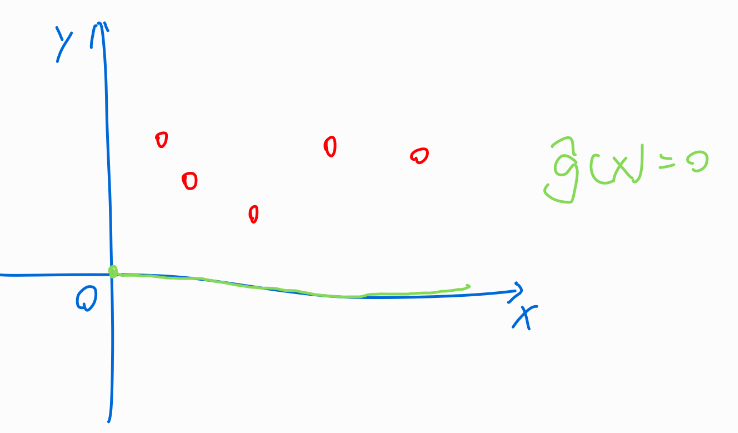
\includegraphics[width=0.3\textwidth]{figs/2a.png}
    \caption{(a)}
    \label{fig:2a}
\end{figure}
\begin{figure}[h]
    \centering
    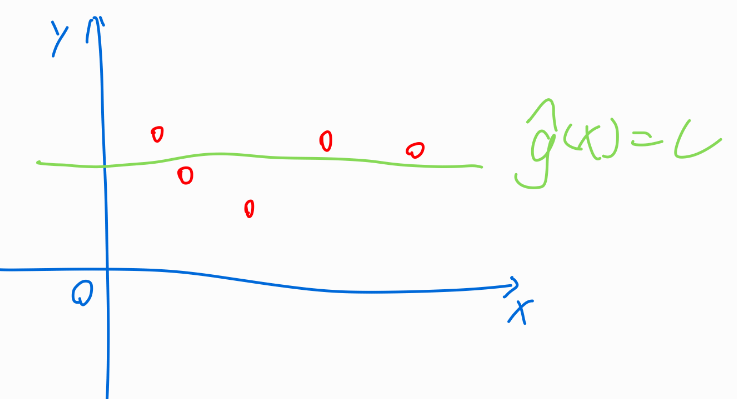
\includegraphics[width=0.3\textwidth]{figs/2b.png}
    \caption{(b)}
    \label{fig:2b}
\end{figure}
\begin{figure}[h]
    \centering
    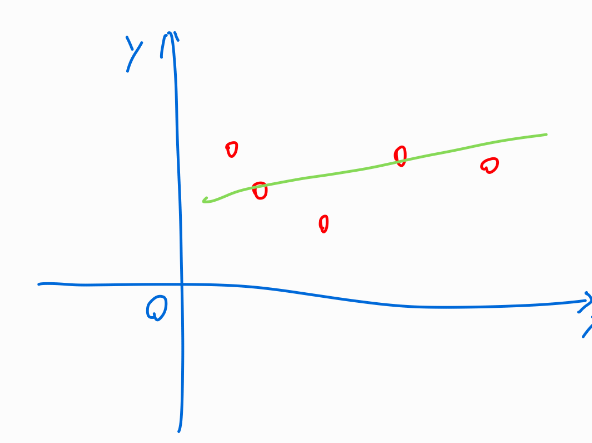
\includegraphics[width=0.3\textwidth]{figs/2c.png}
    \caption{(c)}
    \label{fig:2c}
\end{figure}
\begin{figure}[h]
    \centering
    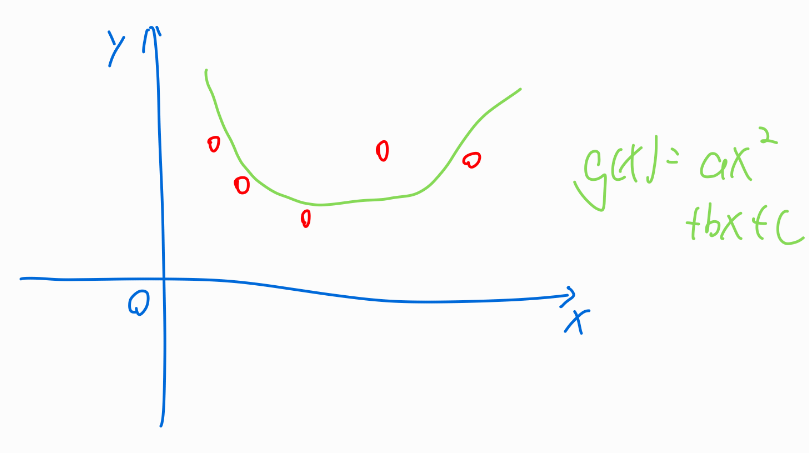
\includegraphics[width=0.3\textwidth]{figs/2d.png}
    \caption{(d)}
    \label{fig:2d}
\end{figure}
\begin{figure}[h]
    \centering
    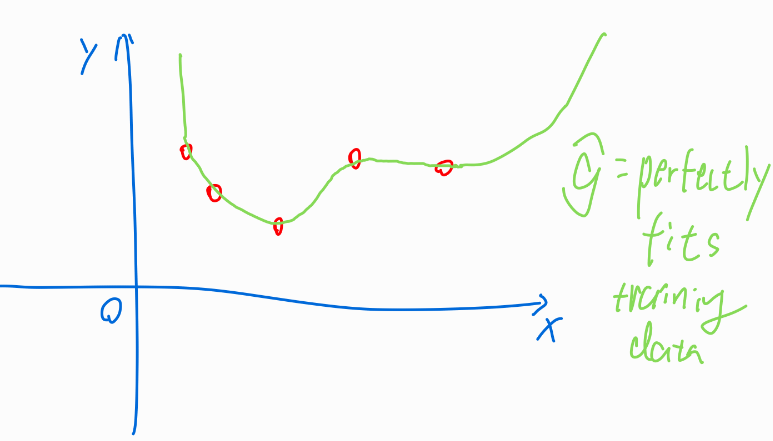
\includegraphics[width=0.3\textwidth]{figs/2e.png}
    \caption{(e)}
    \label{fig:2e}
\end{figure}
\newpage
\section*{Conceptual 3}
\begin{figure}[h]
    \centering
    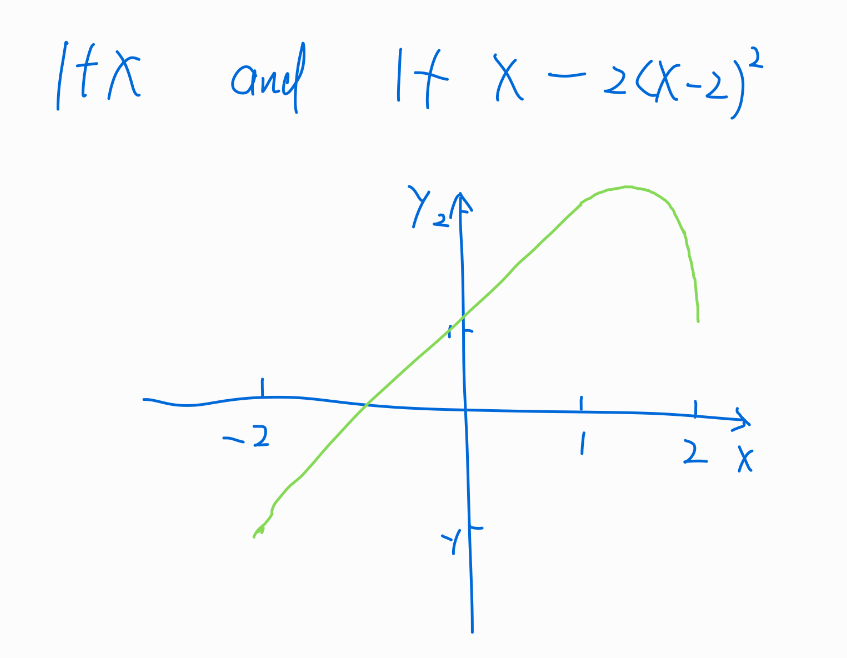
\includegraphics[width=0.5\textwidth]{figs/3.png}
    \caption{3}
    \label{fig:q3}
\end{figure}
\newpage
\section*{Conceptual 5}
\begin{enumerate}[label=(\alph*)]
\item
g2 because it is more flexible and can fit the data better.
\item
cannot be determined. However, if g2 overfits then g1 will perform better.
\item
same since the penalty term 
\end{enumerate}

\newpage
\section*{Applied 6}
\subsection*{a}
\begin{figure}[h]
    \centering
    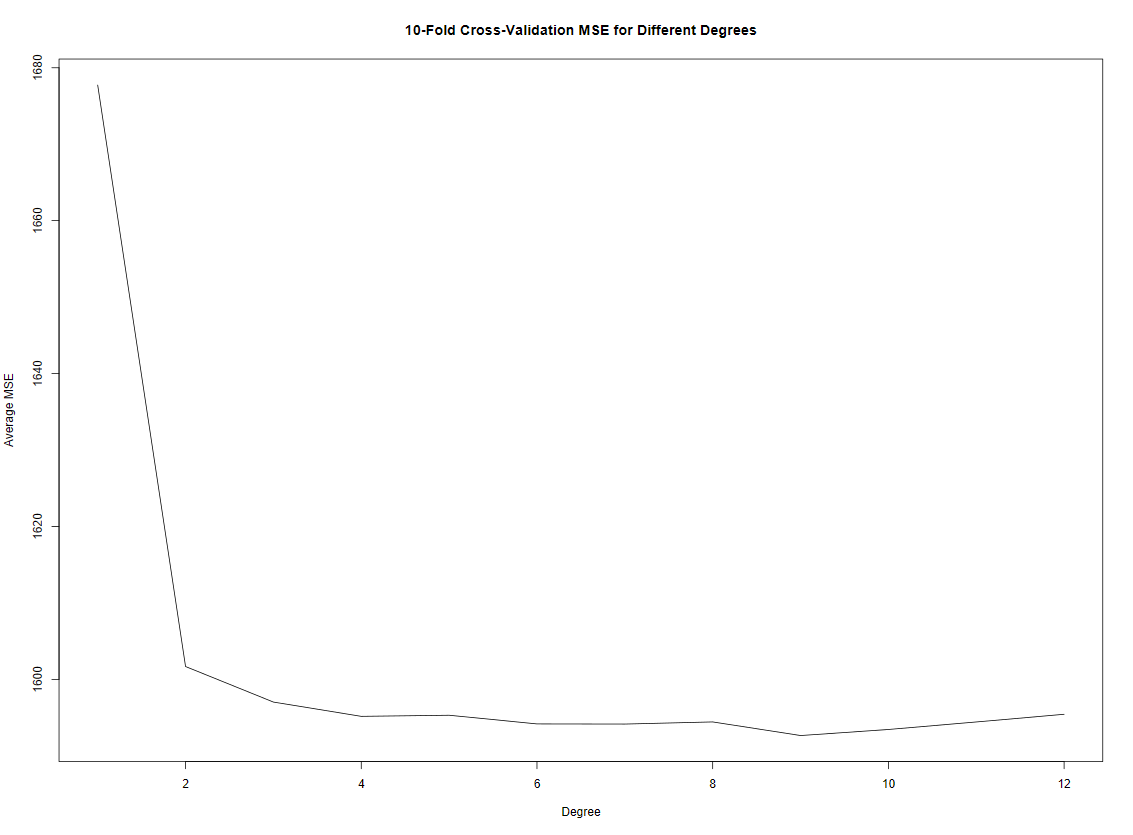
\includegraphics[width=0.5\textwidth]{figs/q6-a1.png}
    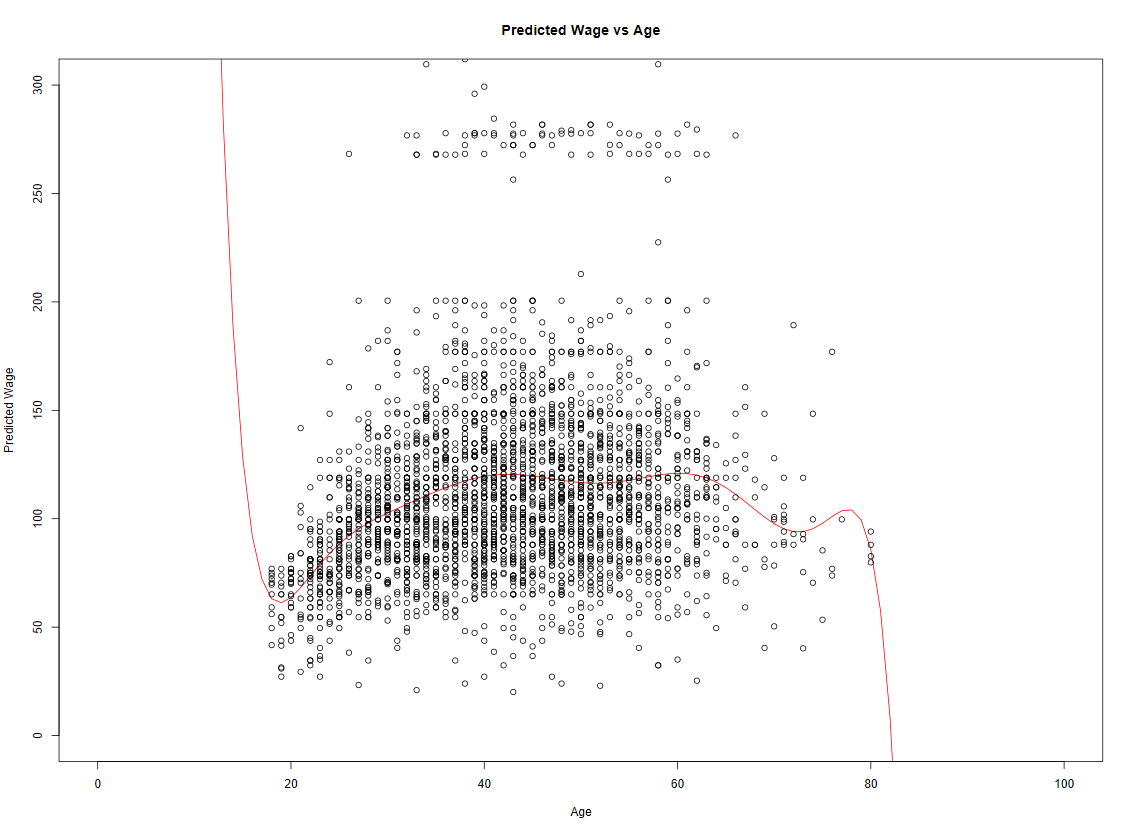
\includegraphics[width=0.5\textwidth]{figs/q6-a2.png}
    \caption{}
    \label{fig: plots}
\end{figure}
\inputminted{r}{src/q6a.R}

\begin{figure}[h]
    \centering
    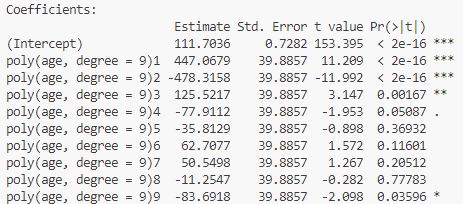
\includegraphics[width=0.5\textwidth]{figs/q6-a3.png}
    \caption{}
    \label{fig: summary}
\end{figure}

\begin{figure}[h]
    \centering
    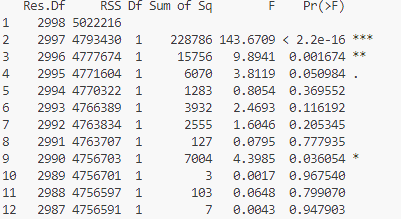
\includegraphics[width=0.5\textwidth]{figs/q6-a4.png}
    \caption{}
    \label{fig: anova}
\end{figure}

\newpage
the best degree is 9.
The anova tests show that only degree 2 3 and 9 significantly improve the degree 1 model.
This is consistent with summary output

\newpage
\subsection*{b}
\begin{figure}[h]
    \centering
    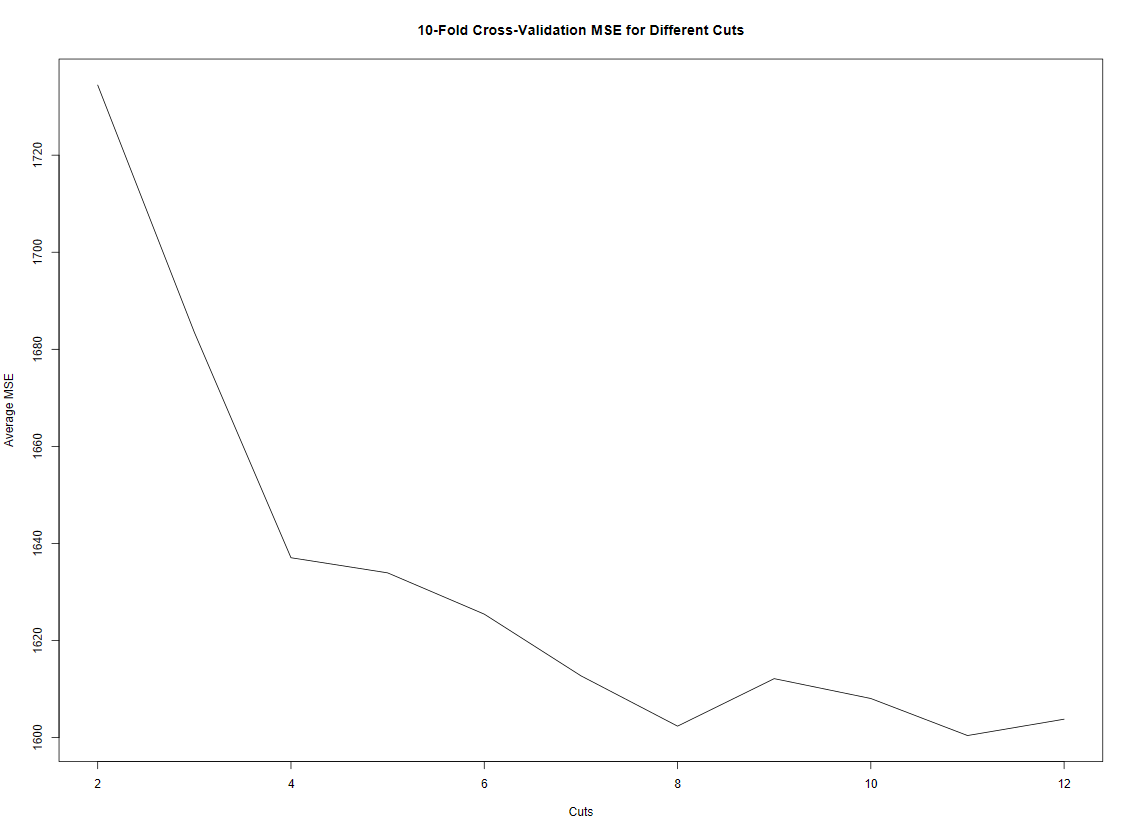
\includegraphics[width=0.5\textwidth]{figs/q6-b1.png}
    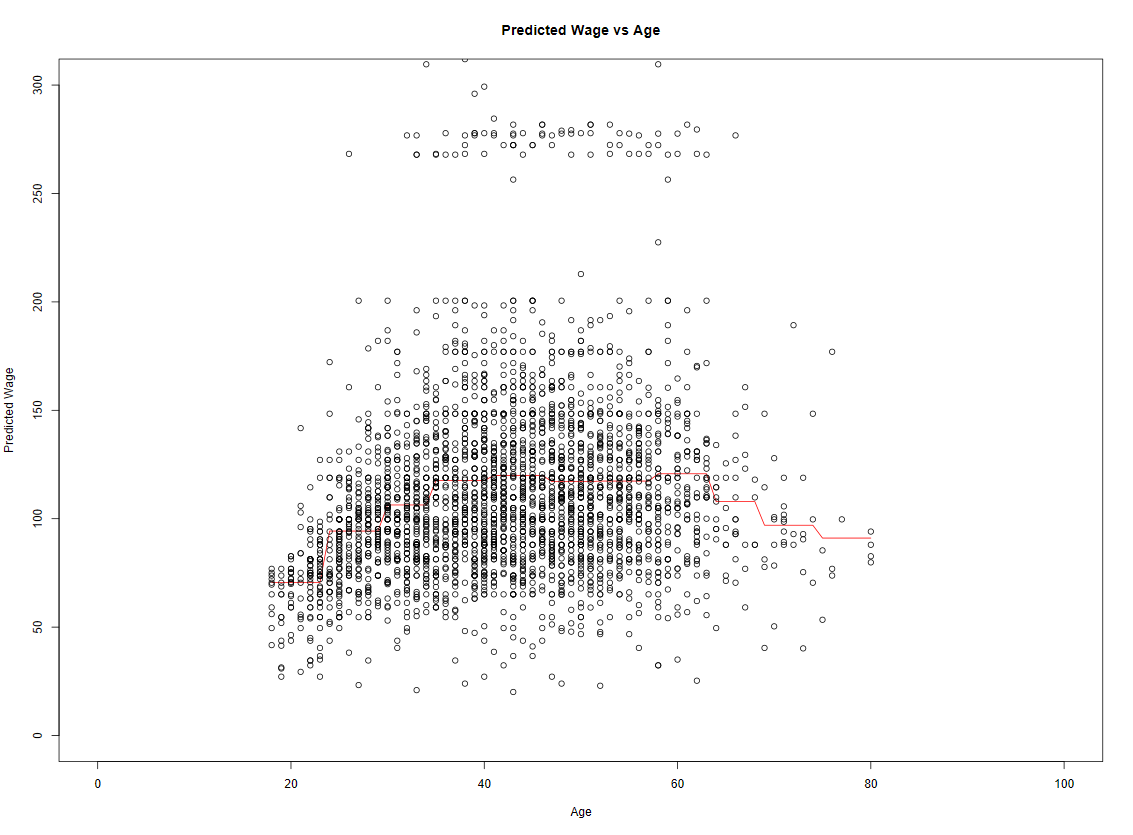
\includegraphics[width=0.5\textwidth]{figs/q6-b2.png}
    \caption{}
    \label{fig: b2 plots}
\end{figure}

\inputminted{r}{src/q6b.R}

The best number of cuts is 11




\newpage
\section*{Applied 8}
\inputminted{r}{src/q8.R}
\newpage
\begin{figure}[h]
    \centering
    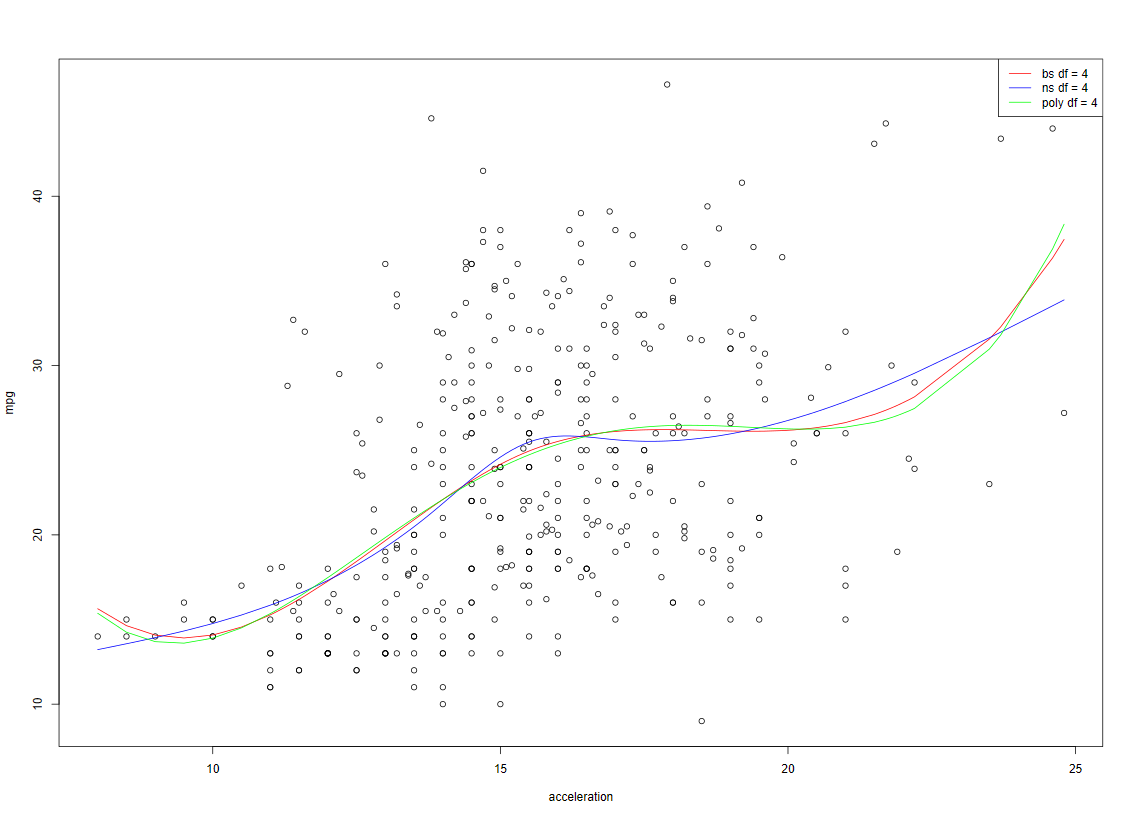
\includegraphics[width=0.6\textwidth]{figs/q8-1.png}
    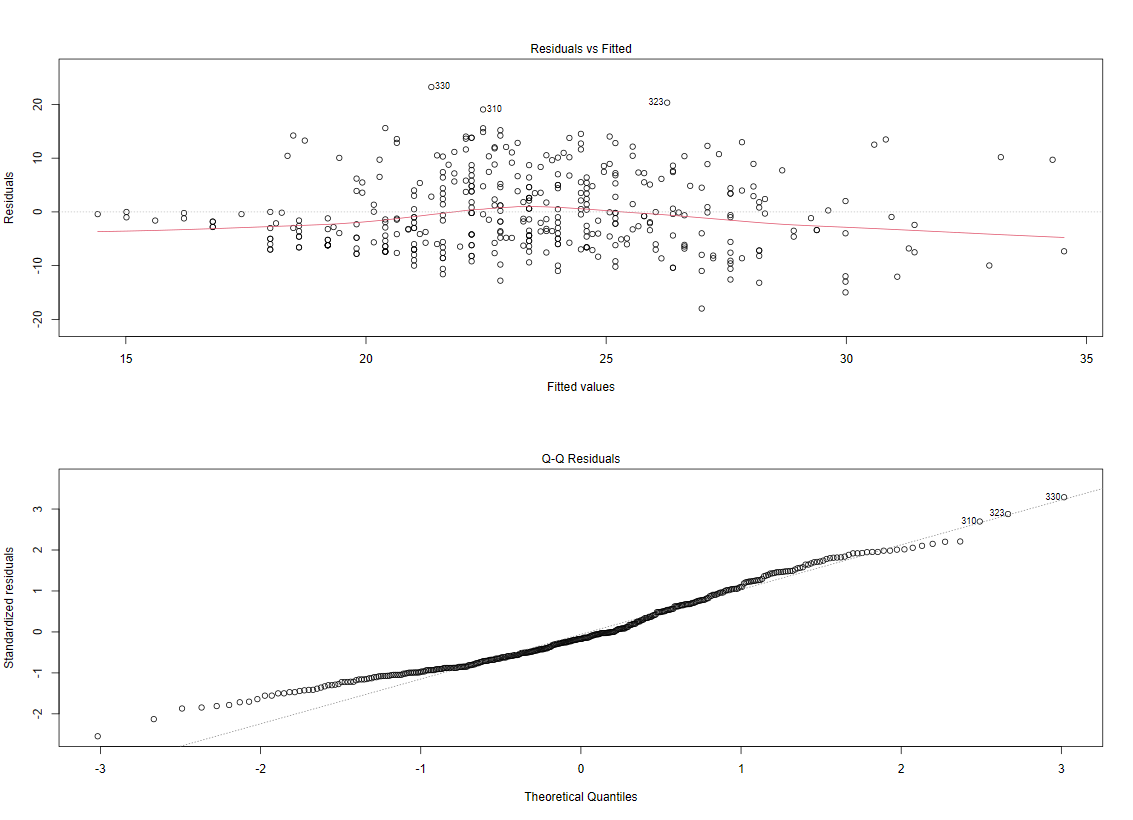
\includegraphics[width=0.6\textwidth]{figs/q8-2.png}
    \caption{}
    \label{fig: q8-1}
\end{figure}

The normality plot shows that the some residuals are not normally distributed.

\newpage
\section*{Applied 9}
\inputminted{r}{src/q9.R}
\subsection*{a, b, c}

\begin{figure}[h]
    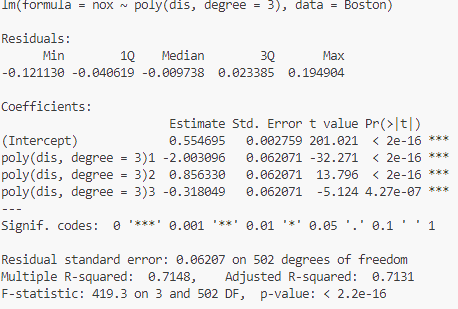
\includegraphics[width=1\textwidth]{figs/q9-11.png}
    \caption{}
    \label{fig: q9-11}
\end{figure}
\begin{figure}[h]
    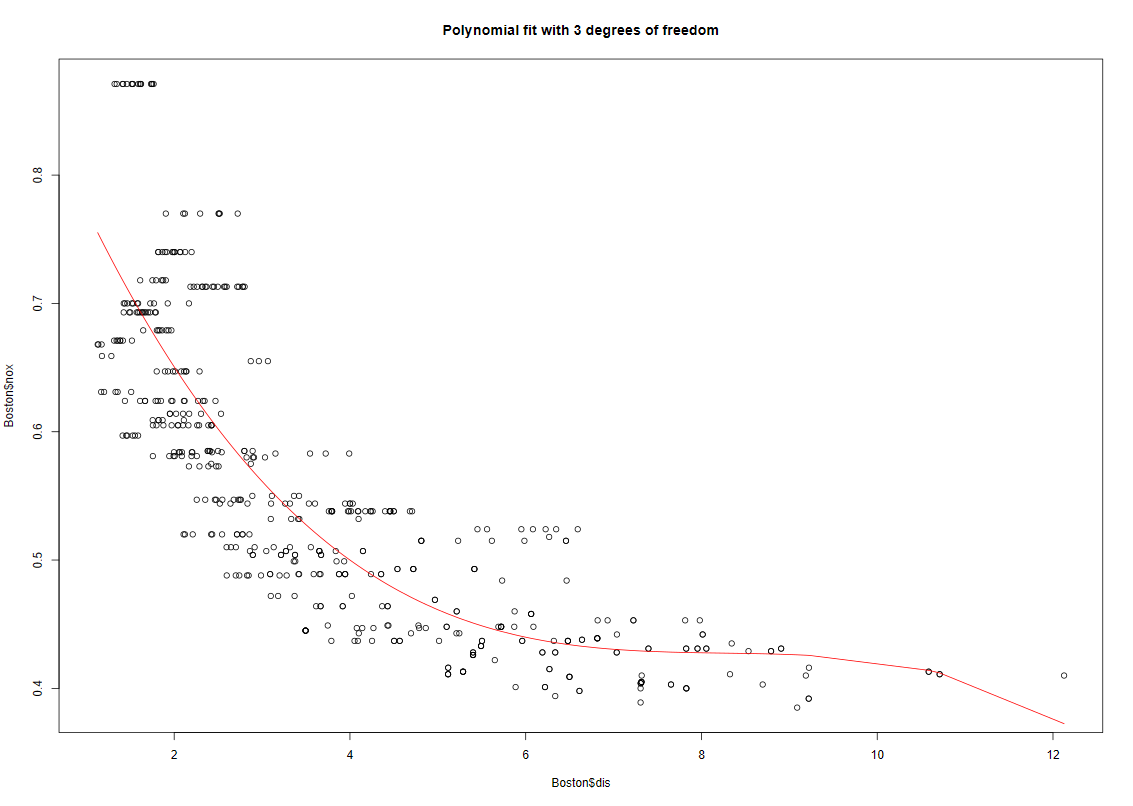
\includegraphics[width=1\textwidth]{figs/q9-12.png}
    \caption{}
    \label{fig: q9-12}
\end{figure}
\begin{figure}[h]
    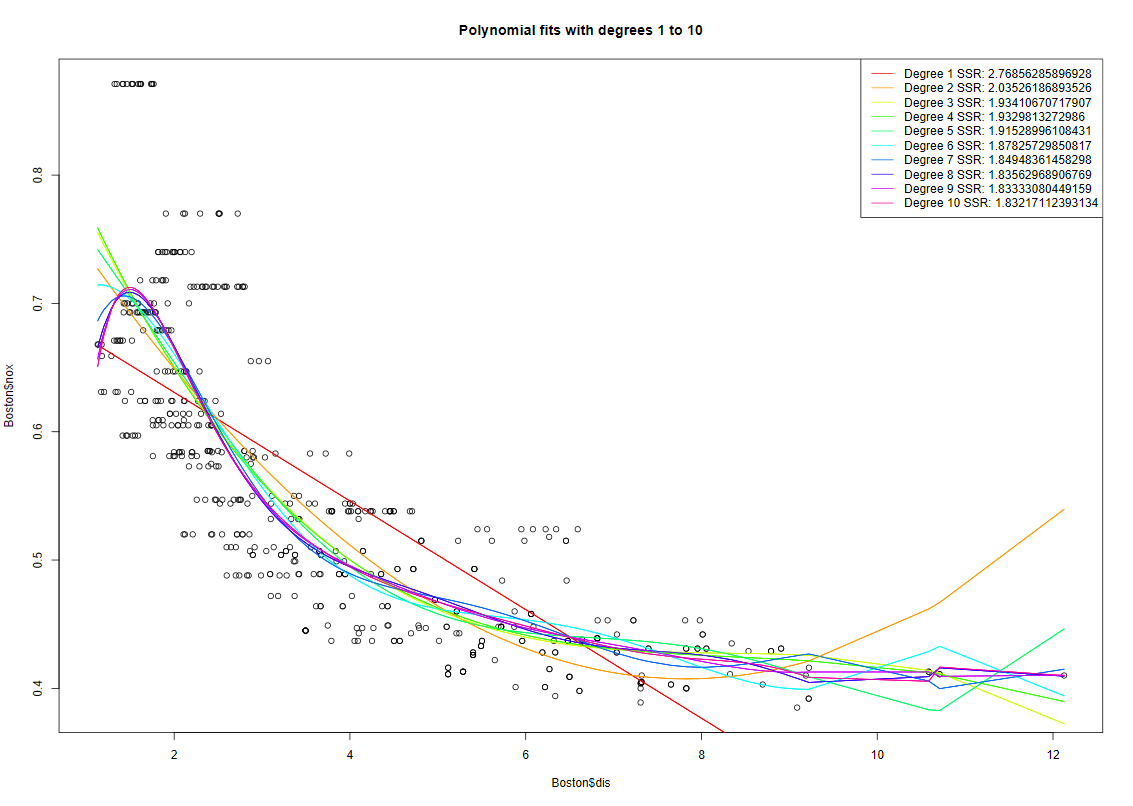
\includegraphics[width=1\textwidth]{figs/q9-13.png}
    \caption{}
    \label{fig: q9}
\end{figure}

The best degree is 3 from 10 folds cross validation with mse as the metric.

\subsection*{d}
\begin{figure}[h]
    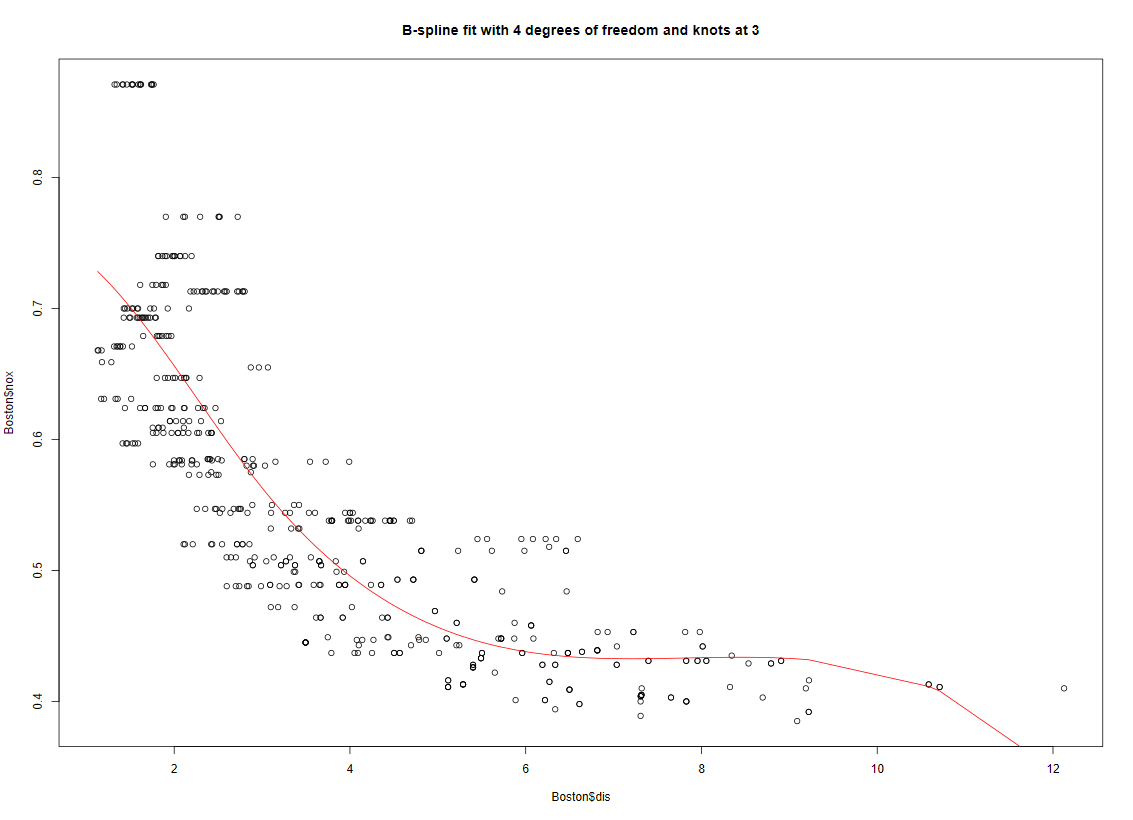
\includegraphics[width=1\textwidth]{figs/q9-2.png}
    \caption{}
    \label{fig: q9-2}
\end{figure}
The knots is chosen at 3 because it is where the curvature of the plot changes.

\subsection*{e, f}
\begin{figure}[h]
    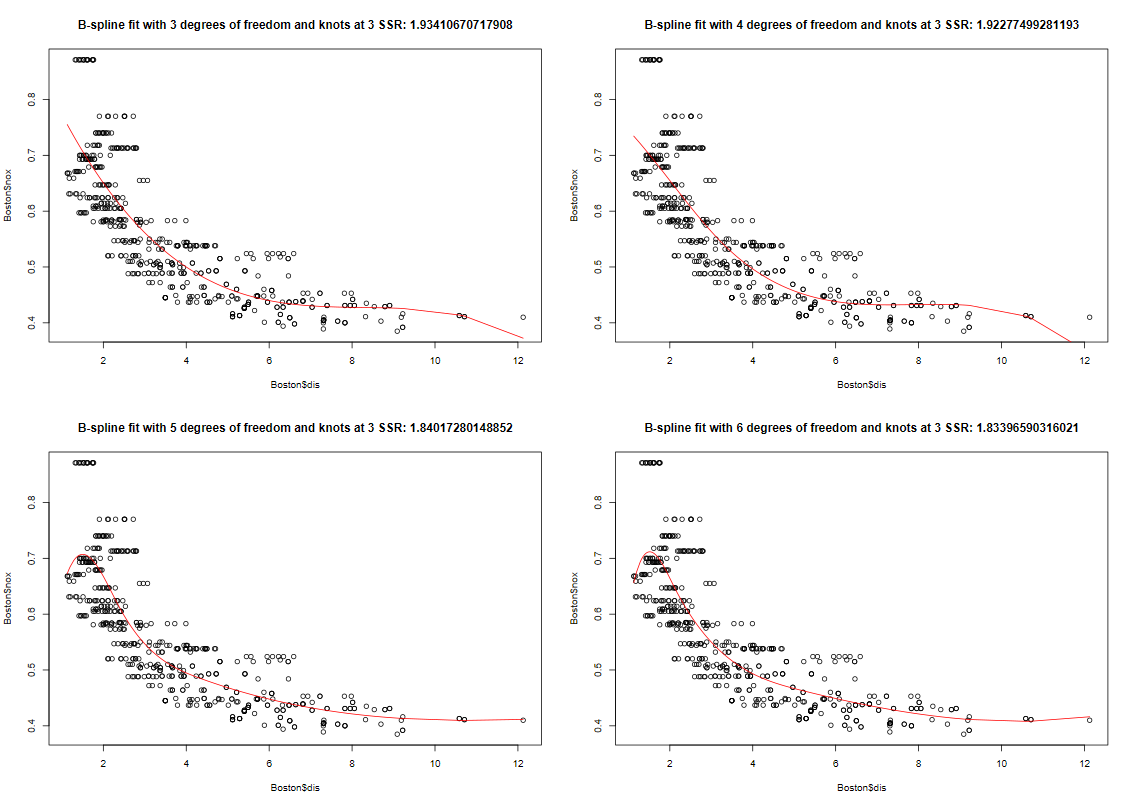
\includegraphics[width=1\textwidth]{figs/q9-3.png}
    \caption{}
    \label{fig: q9-3}
\end{figure}

Higher degrees of freedom leads to overfitting. the change of curvature near x=2 for df > 4 does not reflect the true trend.
\end{document}